\section{Switching Loop}
\subsection{Switching Loop의 개념}
    디바이스 사이에 네트워크 연결경로가 한 개만 있다면, 한 지점에서의 장애로 네트워크 전체가 기능을 상실할 수 있다. 따라서 대부분의 네트워크는 Redundant Topology (이중화 설계)로 네트워크 연결경로를 두 개 이상 설정하여 Error 발생시 안정성을 높인다. 그러나 Redundant Topology로 인해 여러개의 브리지 또는 스위치가 Loop 형태로 연결된다면 Frame이 Loop를 끝없이 순환하는 Switching Loop 현상을 일으킬 수 있다. \\
    스위치는 Frame이 입력되었을때 목적지 MAC 주소가 MAC Table에 없으면 Frame을 복제하여 입력 포트를 제외한 다른 모든 포트로 재전송 (Flooding)하기 때문에 Loop 형태의 Topology에서 무한히 같은 Frame을 주고 받는 Switching Loop가 발생한다. Layer-2 헤더에는 TTL (Time to Live) field가 없기 때문에 Frame이 무한히 loop를 돌면서 네트워크를 마비시킨다. \\
    \vspace{-4mm}
    \begin{figure}[!h]\centering
		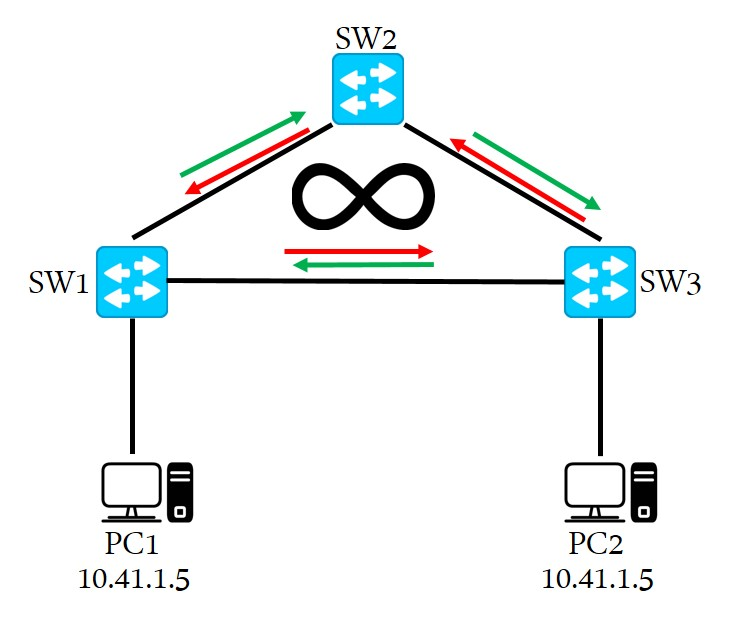
\includegraphics[width=.65\textwidth]{image/week06/1-1.png}
		\caption{\small Switching Loop}
		\vspace{-10pt}
    \end{figure}
    
\subsection{Switching Loop에 의한 현상}
    \begin{enumerate}
        \item Broadcast Storm : ARP 등 Broadcast되는 Frame이 Loop topology에서 끊임없이 돌고 도는 현상
        \item Multi Fame Copies : 단일 Frame이 시계방향과 반대방향으로 돌아 중복되어 수신된다.
        \item MAC Address Table Instability : 프레임이 계속 돌기 때문에 확정적인 MAC Table을 정할 수 없다.
    \end{enumerate}
\newpage